\section{Dispositif: Effet Tcherenkov par des électrons}

Cette manipulation a pour but la caractérisation d'un module optique (OM) développé pour l'expérience AMANDA. Afin d'étudier les propriétés de cet OM, vous devrez mettre au point le dispositif nécessaire à la prise de mesure. Après avoir pris connaissance avec le dispositif, vous serez ainsi amené à développer vous même la logique d'acquisition des données. Vous analyserez ensuite celles-ci grâce aux outils statistiques et informatiques que vous aurez vu en cours. 

Cette manipulation utilise une source de radiation $\beta^+$ composée de Strontium $^{90}$Sr. Les électrons émis par la source traverse ensuite une plaque de quartz d'indice de réfraction  $n = 1.478$. Lors de leur passage, les électrons vont produire un rayonnement Tcherenkov qui pourra être détecté par l'OM. Dans ce dispositif, l'OM se trouve à une position fixe située à un angle de 45$^{\circ}$ par rapport à la direction d'émission des électrons. La source radioactive est combinée à un spectromètre qui va nous permettre de sélectionner l'énergie cinétique des électrons afin de récolter un maximum de rayonnement Tcherenkov dans l'OM. Pour déterminer l'intensité du courant à fournir au spectromètre pour obtenir des électrons de cette énergie, vous devrez d'abord résoudre l'exercice 2.\\

Une fois cette valeur trouvée, vous pouvez allumer le spectromètre. Ce spectromètre est calibré sur la partie descendante de la courbe d'hystérèse, il vous faudra donc respecter les conditions d'utilisations décrites ci-dessous.\\

\textbf{Mode d'emploi du spectromètre :}
\begin{quote}
    \begin{itemize}
        \item Démarrez à $I$ = 0 A
        \item Aller à saturation $I$ $\sim$ 2,6 A
        \item Descendre à la valeur $I_t$ désirée
    \end{itemize}
\end{quote}
\textbf{Remarque :} Si on veut changer $I_t$ pour une valeur plus petite, on descend vers cette valeur. En revanche, si on veut augmenter cette valeur, on doit recommencer le cycle d'hystérèse. 

\begin{figure}[!h]
    \centering
    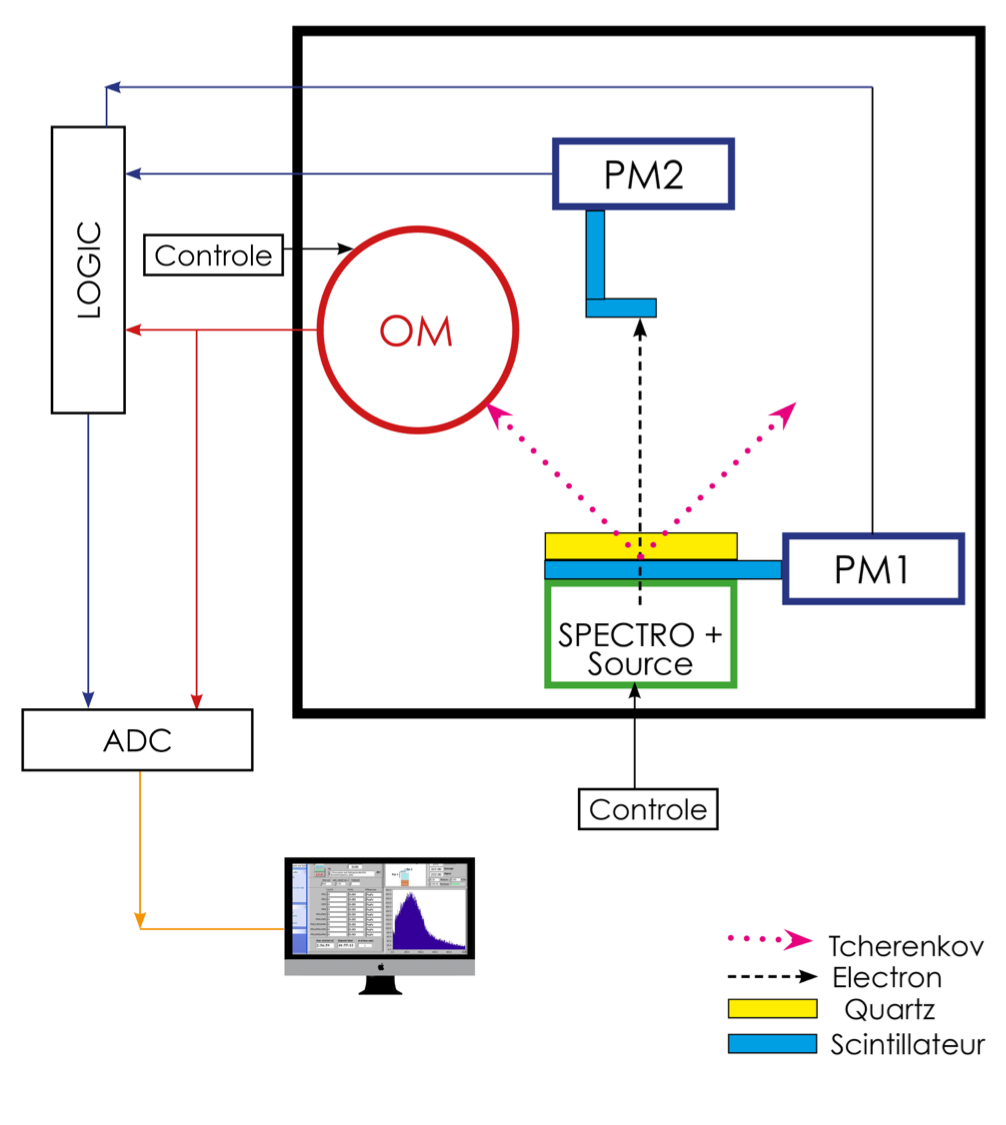
\includegraphics[width=0.5\textwidth]{figures/Dispositif_1.png}
    \caption{Dispositif expérimental de l'effet Tcherenkov produit par des électrons.}
    \label{fig:dispo1} 
\end{figure}

Dans ce dispositif, sont également présent 2 photo-multiplicateurs (PMs) chacun relié à un scintillateur. Le premier (PM1) est situé entre la source et la plaque de quartz et nous permet de vérifier qu'un électron a été émis par la source. Le second PM confirme que l'électron a bien traversé le quartz. Ces PMs ont donc pour but d'assurer que le signal détecté par l'OM est en coïncidence avec un électron qui a produit des photons Tcherenkov.


\subsection{Exercices Pr\'eparatoires}

\subsubsection{Exercice 1}
Sachant que l'OM est placé à un angle de $45^\circ$ par rapport à la direction d'émission des électrons ($m_\mathrm{e} = 0.511$\,MeV/$c^2$) de la source de strontium, à quel courant faut-il régler le spectromètre pour récolter un maximum de rayonnement Tcherenkov dans l'OM, sachant que l'indice de réfraction du quartz est de $1.478$?\\

Le graphique suivant vous donne la relation entre l'énergie cinétique des électrons et l'intensité du courant.

\begin{figure}[!h]
    \center{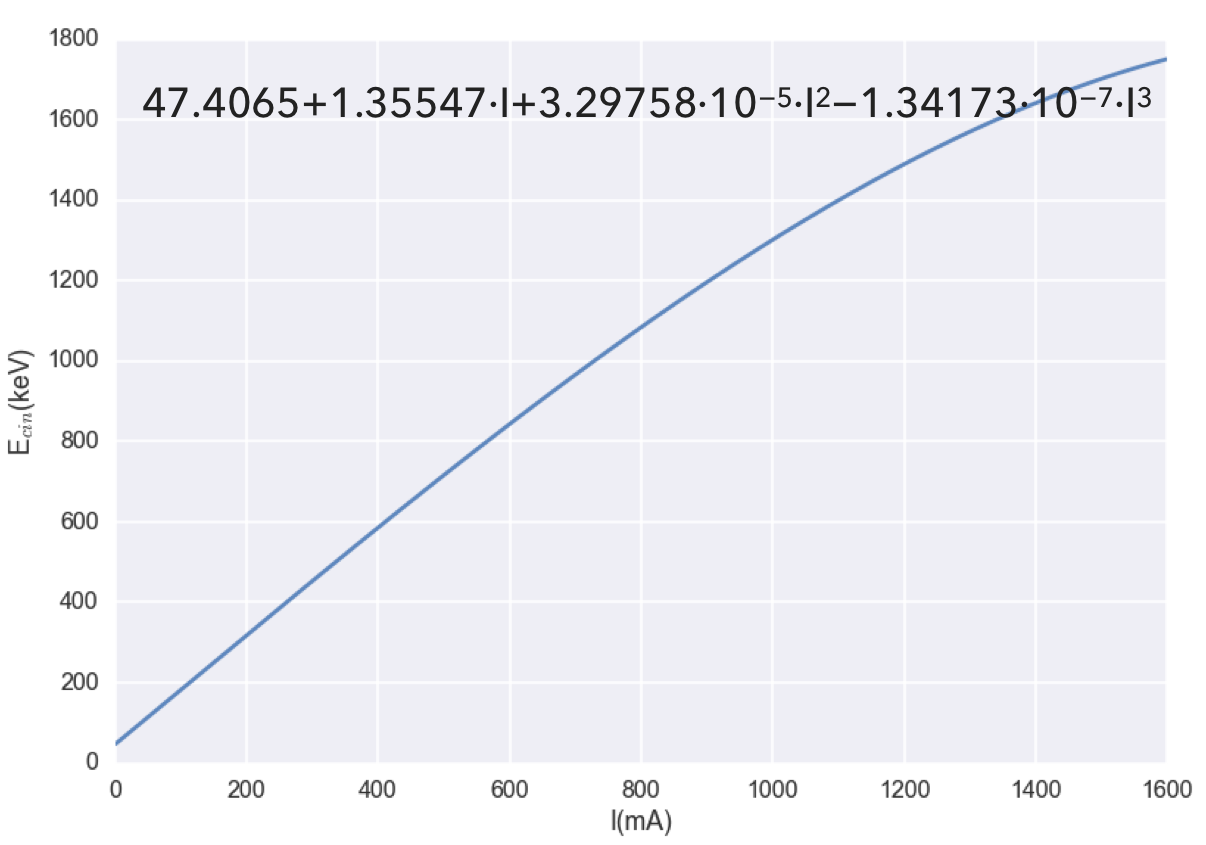
\includegraphics[width=0.5\textwidth]
    {figures/Relation_Ecin_I.png}}
    \caption{\label{fig:spectro} Relation entre l'intensité du courant fourni au spectromètre et l'énergie cinétique des électrons.}
\end{figure}

\ifthenelse{\boolean{showAdditional}}{
\begin{additional}
\begin{align*}
\beta &= \frac{1}{n\cos\Theta_\mathrm{c}} = 0.9568\\
 &= \frac{pc}{E}\\
 &= \frac{\sqrt{E^2-m_\mathrm{e}^2c^4}}{E}\\
 &\\
E &= \sqrt{\frac{m_\mathrm{e}^2c^4}{1 - \beta^2}} = 1.7575\,\mathrm{MeV}\\
E_\mathrm{cin}&=E- m_\mathrm{e}\\
 &= 1.247\,\mathrm{MeV} \\
&\Rightarrow \boxed{I \approx 950\,\mathrm{mA}} \\
\end{align*}
\end{additional}
}

\subsubsection{Exercice 2}
Calculer l'ordre de grandeur du nombre de photons \'emis entre $350$ et $500$\,nm par un 'electron de $1247$\,keV d'\'energie cin\'etique traversant une fen\^etre de quartz de 1\,mm d'\'epaisseur, sachant que pour ce domaine de longueurs d’onde, l'indice de r\'efraction du quartz varie de moins de 1\% et peut \^etre consid\'er'e constant ($1.478$). N\'egliger la perte d'\'energie de l'\'electron dans le quartz.\\ $\alpha = 1/137$

\ifthenelse{\boolean{showAdditional}}{
\begin{additional}
Formule de \emph{Frank-Tamm}:
\begin{align*}
\frac{\mathrm{d}N}{\mathrm{d}x} &= \int_{\lambda_0}^{\lambda_1} \frac{2\pi\alpha z^2}{\lambda^2} \sin^2\Theta_\mathrm{c} \mathrm{d}\lambda\\
&=\frac{\pi}{137}\int_{350\,\mathrm{nm}}^{500\,\mathrm{nm}}\frac{\mathrm{d}\lambda}{\lambda^2}\\
N&=\frac{\pi}{137}\cdot\left(\frac{1}{350\,\mathrm{nm}}-\frac{1}{500\,\mathrm{nm}}\right)\cdot1\,\mathrm{mm}\\
&=\boxed{19.65}
\end{align*}
\end{additional}
}

\subsubsection{Exercice 3}
En supposant que le diam\`etre du collimateur plac\'e devant la photocathode de l'OM est de 6 cm et qu'il se trouve \`a 17\,cm de la fen\^etre de quartz, combien de photoelectrons l'OM peut-il enregistrer par \'electron de la source, en supposant la transmittance $T$ \`a 90\%, l'efficacit\'e quantique est de $\epsilon_\mathrm{q}=15\%$?

\ifthenelse{\boolean{showAdditional}}{
\begin{additional}
Avec $N_\mathrm{\gamma}^{\mathrm{quartz}}$ trouv\'e avant, on obtient:
\begin{align*}
N_{\mathrm{pe}} &= \epsilon_\mathrm{q} \cdot T \cdot N_\mathrm{\gamma}^{\mathrm{OM}}\\
 &= \epsilon_\mathrm{q} \cdot T \cdot \frac{6\,\mathrm{cm}}{2\pi \cdot 17\,\mathrm{cm} \cdot\sin\Theta_\mathrm{c}} \cdot N_\mathrm{\gamma}^{\mathrm{quartz}}\\
&= \boxed{3.58}
\end{align*}
\end{additional}
}


\subsection{Prise de mesure}

Pour cette manipulation, il vous est demandé de préparer le dispositif expérimental nécessaire à la prise de mesure. Cela implique, dans un premier temps, de :

\begin{center}
\fbox{
\begin{minipage}{0.75\textwidth}
\textbf{Se familiariser avec le dispositif :} 
\begin{quote}
\begin{itemize}
\item vérifier le signal des différents PMs et de l'OM
\item étudier l'efficacité des PMs
\item calibrer l'ADC
\item développer la logique d'acquisition de données
\item mesurer le bruit de fond
\end{itemize}
\end{quote}
\end{minipage}
}
\end{center}

\subsubsection{Vérification du dispositif}
A l'aide de l'oscilloscope, vérifiez le signal provenant des différents photo-multiplicateurs (PMs) et de l'OM. Transformez ensuite votre signal analogue en signal digital à l'aide du discriminateur et observez celui-ci sur l'oscilloscope.

\subsubsection{Mesure de l'efficacité}

Il vous est ensuite demandé de mesurer l'efficacité d'un des PMs présents dans votre dispositif. Vous devrez faire cette mesure en faisant varier dans un premier temps le seuil du PM pour lequel vous mesurer l'efficacité. Une fois la valeur optimale du seuil trouvée, répétez le processus en faisant cette fois varier la tension appliquée sur le PM en question. Pour ces deux mesures, veillez également à mesurer le taux d'évènements détectés par le PM dont vous mesurez l'efficacité. Pour effectuer ces mesures, vous avez à votre disposition un scaler NIM.

\ifthenelse{\boolean{showAdditional}}{
\begin{additional}
\begin{itemize}
\item Mesure de l'efficacité de PM1
\item Logique : (PM1 \& PM2 \& OM) et (PM2 \& OM)
\item Mesure du rate de PM1
\end{itemize}
\end{additional}
}

\subsubsection{Calibration de l'ADC}

Nous allons à présent procéder à la calibration du convertisseur analogique-numérique (ADC ou Analogue-to-Digital Converter). En effet, l'ADC vous donne des valeurs en ADC channel, il vous faut donc connaître à quelle charge équivaut un ADC channel.\\

Pour cette calibration, il faut fournir une charge connue et constante à l'ADC. Pour cela, vous avez à votre disposition un générateur de courant continu.

\ifthenelse{\boolean{showAdditional}}{
\begin{additional}
\begin{itemize}
    \item Charge de l'ADC de l'ordre du pC $\to$ $Q\sim100$\,pC 
    \item Utilisation d'une résistance: $U = RI$ avec $R = 2.2$\,k$\mathrm{\Omega}$
    \item Sachant que $Q = I\mathrm{\Delta}t$, déterminer $\mathrm{\Delta}t$
    \item Le gate est ensuite créé à l'aide du dual-timer
\end{itemize}
\end{additional}
}

\subsubsection{Prise de données}

Afin de prendre les données nécessaires à la caractérisation de l'OM, nous devons réfléchir à la logique d'acquisition. Nous allons utiliser l'ADC que nous venons de calibrer et lui fournir le signal de l'OM ainsi qu'une porte logique (gate). Pour créer ce gate, nous avons besoin des modules logiques. Il nous faut réfléchir aux conditions dans lesquelles ont veut déclencher la prise de mesure. En d'autres termes, quand-est-ce que le signal de l'OM nous intéresse? Une fois que cela est clair, vous pouvez l'implémenter à l'aide des modules logiques. Il vous faudra ensuite vérifier que le signal de l'OM et votre porte logique sont en coïncidence à l'aide de l'oscilloscope. Lorsque vous avez effectué cette vérification, reliez le gate et le signal de l'OM à l'ADC pour commencer la prise de mesure.\\

\textbf{Remarque :} Ayant plus d'évènements, la prise de mesure pour la manipulation utilisant les électrons est plus rapide. De ce fait, il vous sera demandé d'effectuer plusieurs mesures en faisant varier la tension. Que cela va-t-il influencer? \\

\textbf{Attention :} Pour la manipulation utilisant les muons, veillez à changer le nom du fichier pour ne pas qu'il soit écrasé lors de la prise de mesure suivante.

\ifthenelse{\boolean{showAdditional}}{
\begin{additional}
\begin{itemize}
\item \textbf{Gate :} PM1 \& PM2 \& OM
\item Faire passer le gate dans le dual-timer pour avoir des fenêtres de tailles constantes
\item Vérifier que l'OM est en même temps que le gate
\item Donner les deux infos à l'ADC et prendre les mesures
\item Prendre des mesures en fonction de la tension pour voir la variation de la position du pic de 1 pe
\end{itemize}
\end{additional}
}

\subsubsection{Mesure du bruit de fond}

Intéressons nous au bruit de fond présent dans ces deux manipulations. Nous voulons connaître le taux de fausses coïncidences, càd les cas où l'OM nous envois un signal qui n'est pas dû à un photon Tcherenkov alors que notre porte logique s'est déclenchée. \\

Dans un premier temps, il vous faut réfléchir à la manière dont vous pouvez implémenter la prise de mesure du bruit de fond. Une fois cette méthode mise en place, vous pouvez démarrer l'acquisition du bruit de fond. A l'aide de l'oscilloscope, pensez toutefois à vérifier que le signal de l'OM et votre gate arrivent en même temps à l'ADC.

\ifthenelse{\boolean{showAdditional}}{
\begin{additional}
\begin{itemize}
\item \textbf{Gate :} PM1 \& PM2 \& OM$_{\mathrm{couvert}}$
\item L'OM n'étant pas fixé au reste du dispositif, il est possible de le séparer physiquement à l'aide d'une couverture
\end{itemize}
\end{additional}
}

\subsection{Analyse de donn\'ees}

A pr\'esent, nous pouvons nous concentrer sur l'analyse des donn\'ees dans le but de caract\'eriser l'OM.

En vous basant sur les donn\'ees, vous devrez calculer:
\begin{center}
\fbox{
\begin{minipage}{0.75\textwidth}
\textbf{Dispositif muon :}
\begin{itemize}
\item le gain $G$ de l'OM,
\item la r\'esolution $\sigma_\mathrm{G}$ de l'OM,
\item le nombre moyen de photo-\'electrons $\langle n_{\mathrm{pe}}\rangle$ produit par trigger dans l'OM.
\end{itemize}
\end{minipage}
}
\end{center}

\ifthenelse{\boolean{showAdditional}}{
\begin{additional}
\textbf{Validation de la procedure d'adjustement:}\\
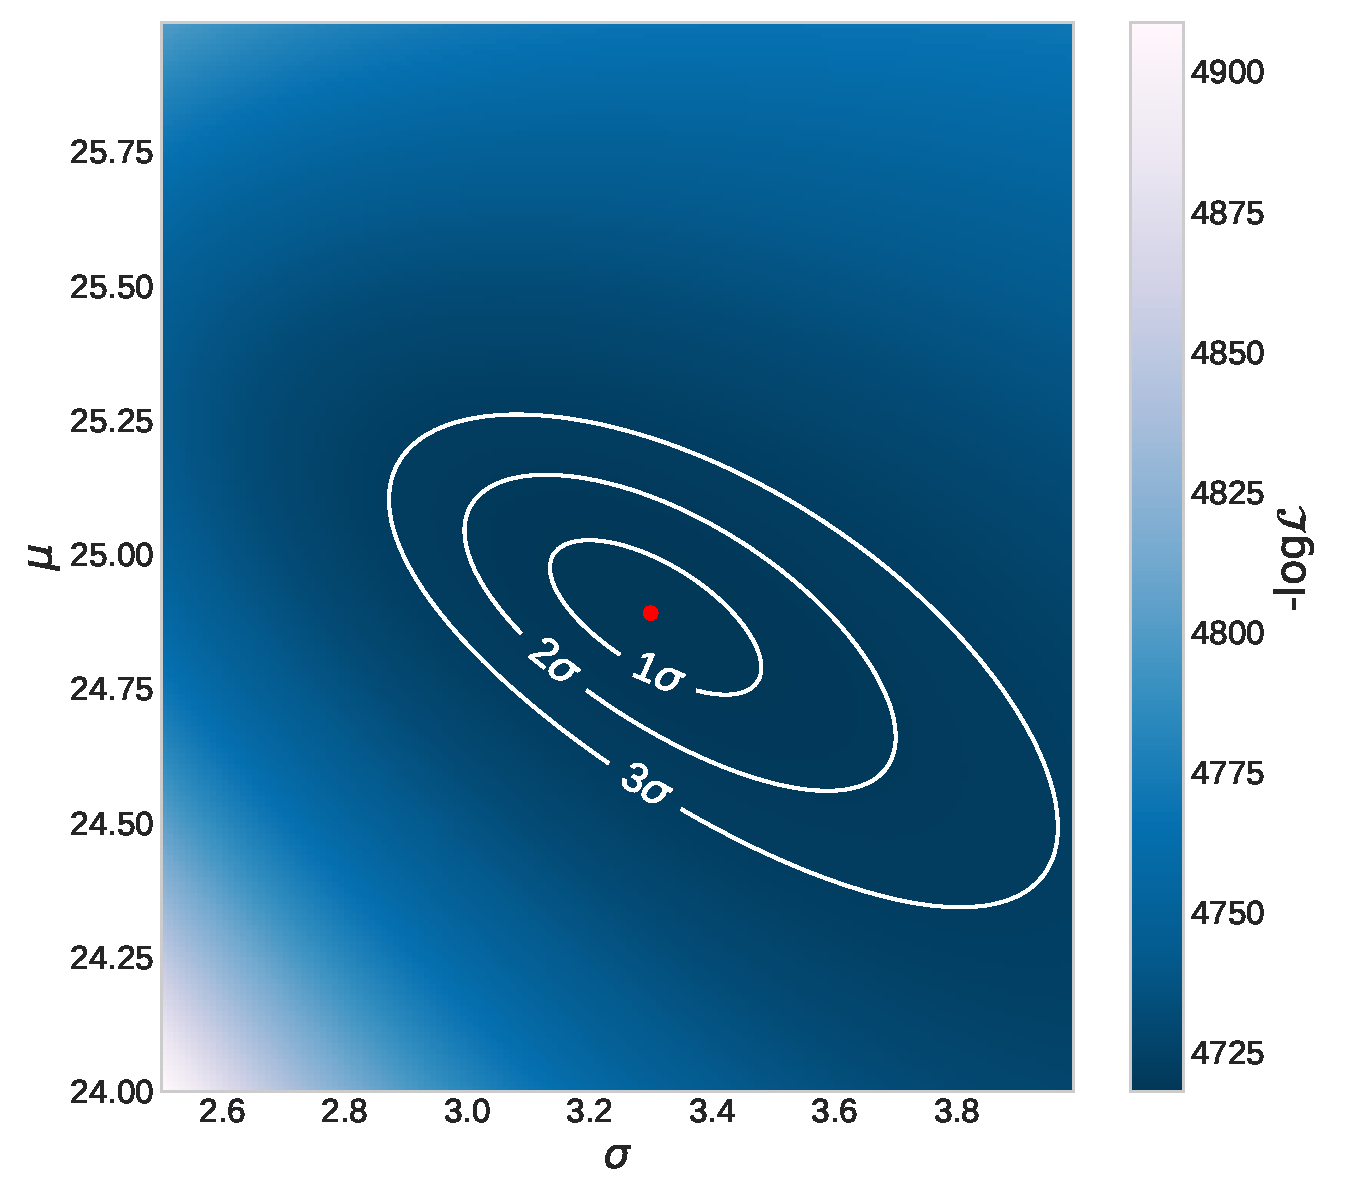
\includegraphics[width=0.45\textwidth]{exampleAnalysis/plots/Likelihood_MC.pdf}
\hfill 
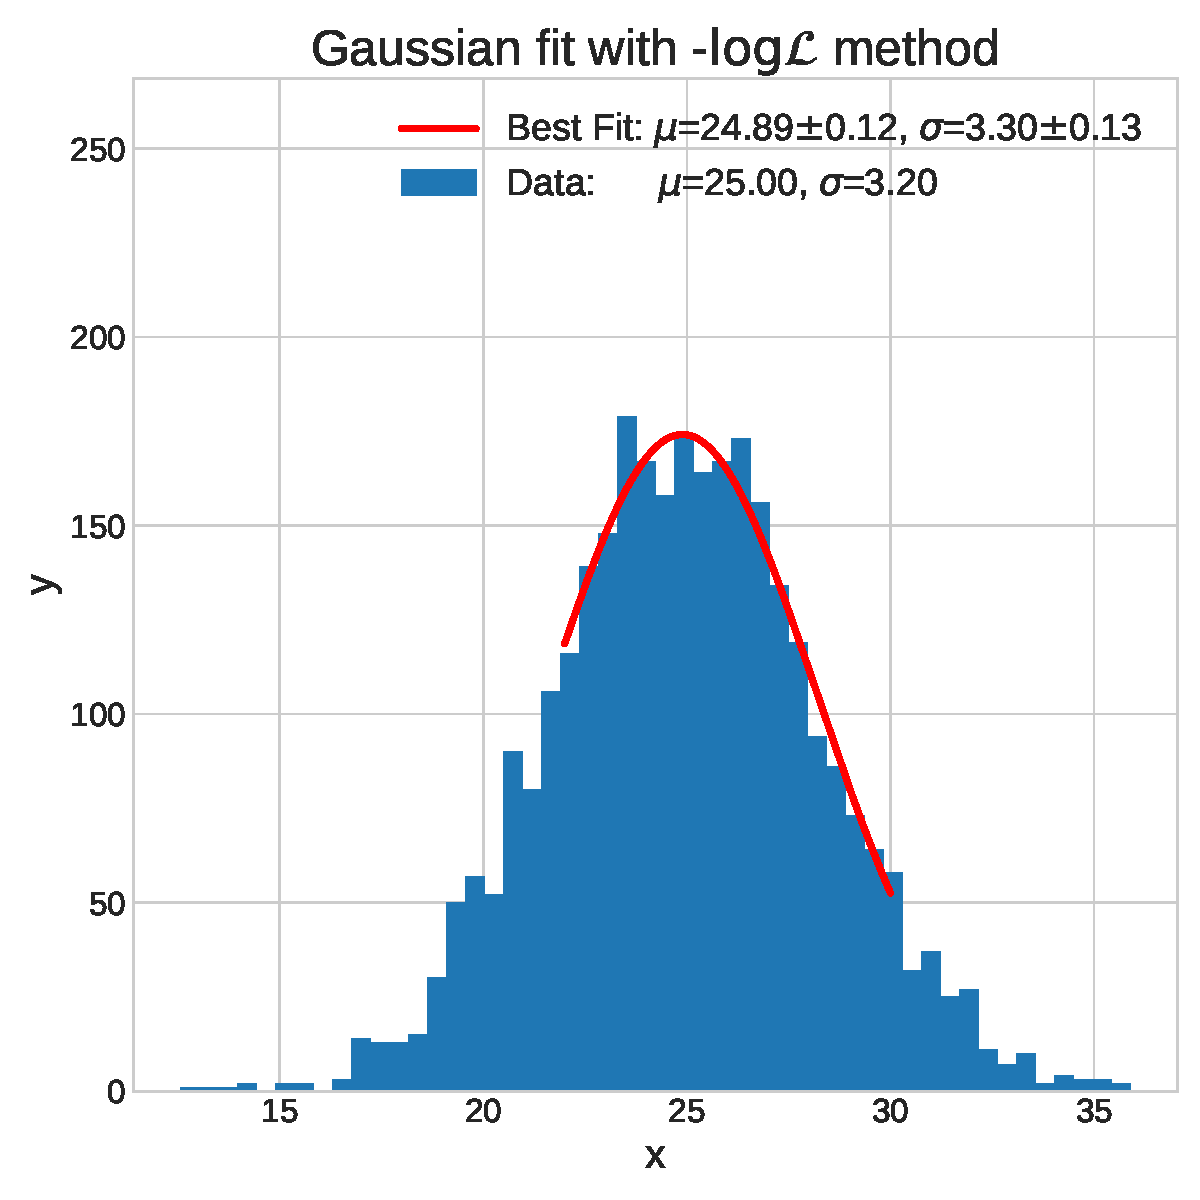
\includegraphics[width=0.45\textwidth]{exampleAnalysis/plots/LLH_Fit_MC.pdf}\\

\textbf{Ajustement des donn{\'e}es:}\\
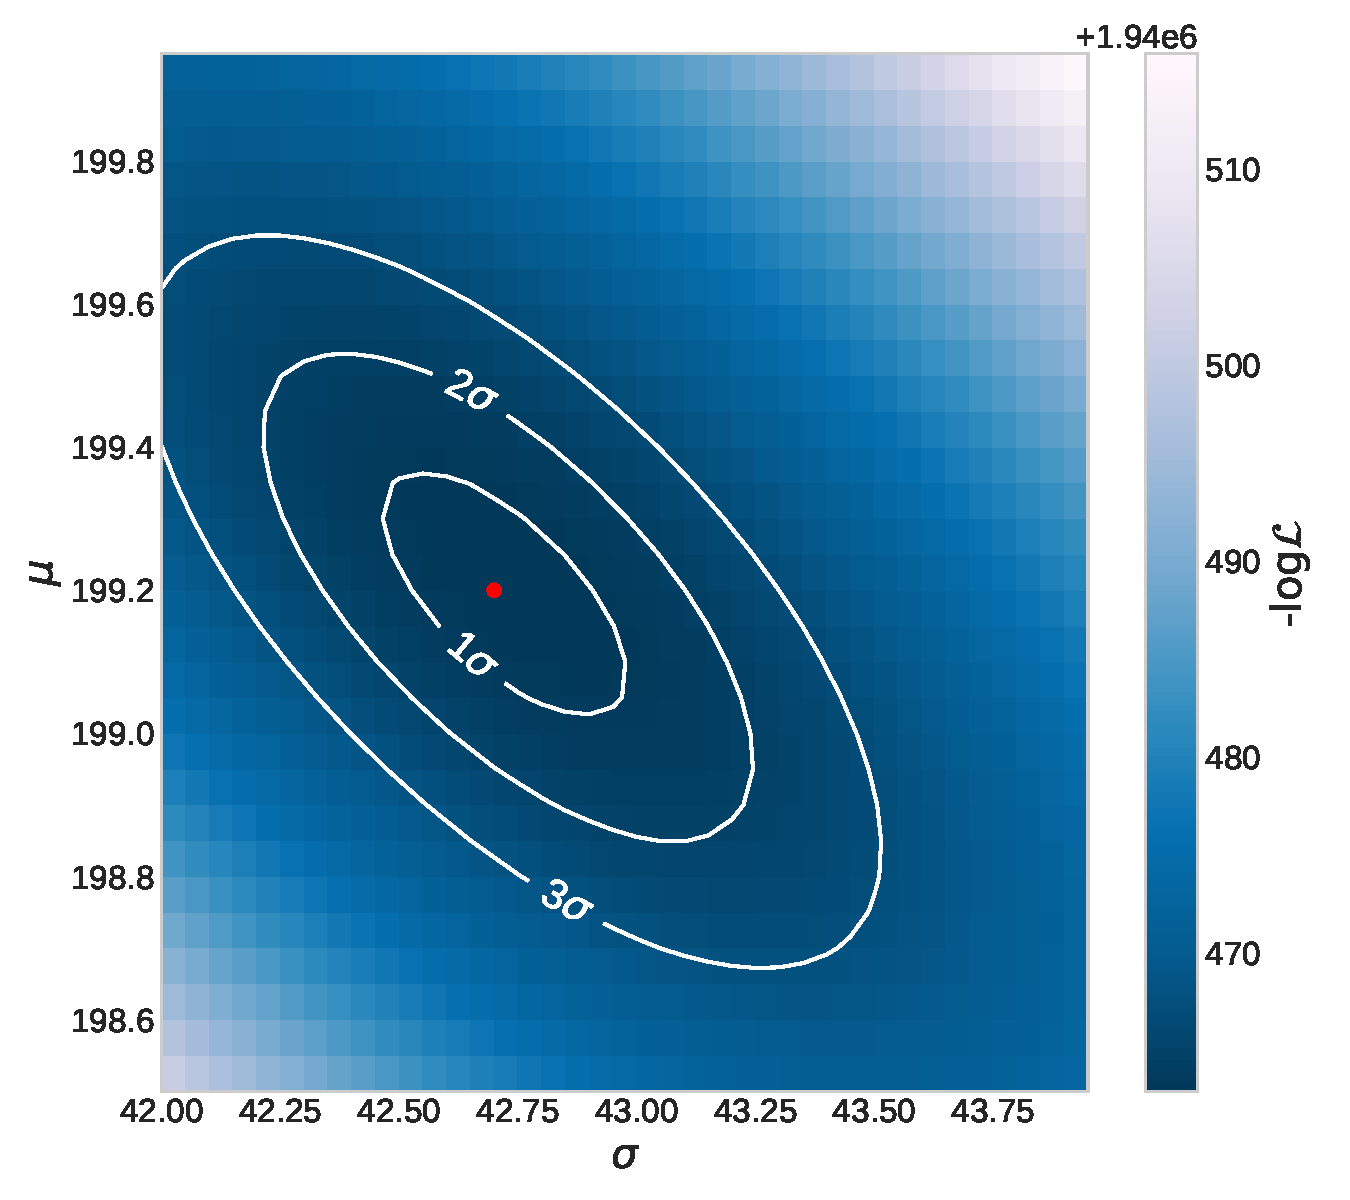
\includegraphics[width=0.45\textwidth]{exampleAnalysis/plots/Likelihood_Data_electron_VME.pdf}\hfill
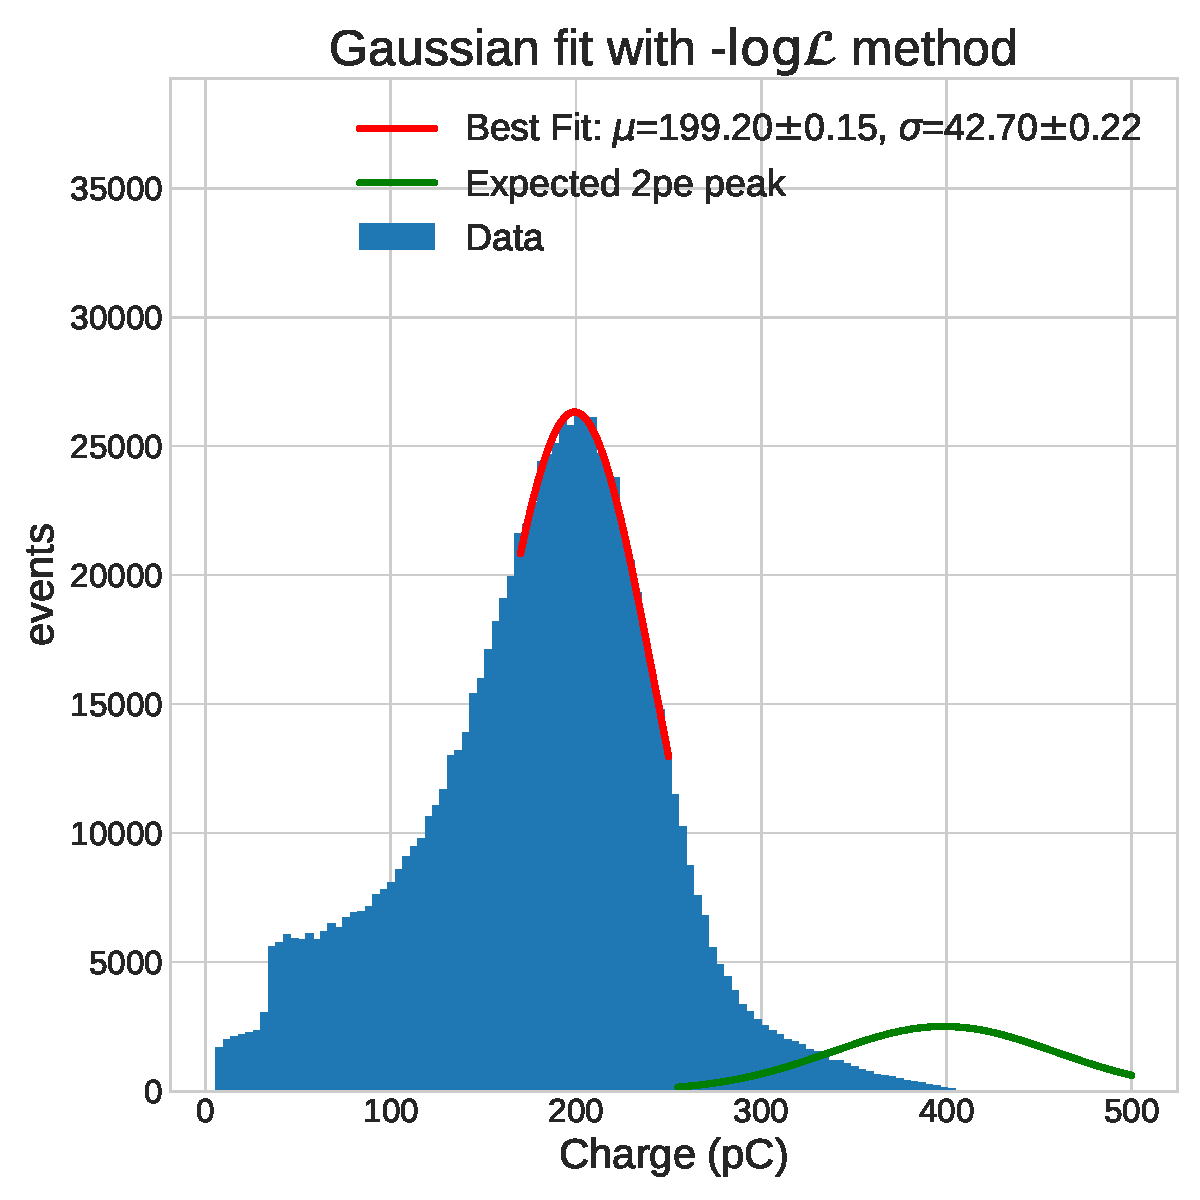
\includegraphics[width=0.45\textwidth]{exampleAnalysis/plots/LLH_Fit_electron_VME.pdf}
\begin{align*}
G &= \mu_{\text{best}}/e = 1242670 \\
\sigma_G &= \sigma_{\text{best}} / \mu_{\text{best}} = 21.44\%
\end{align*}
{\centering
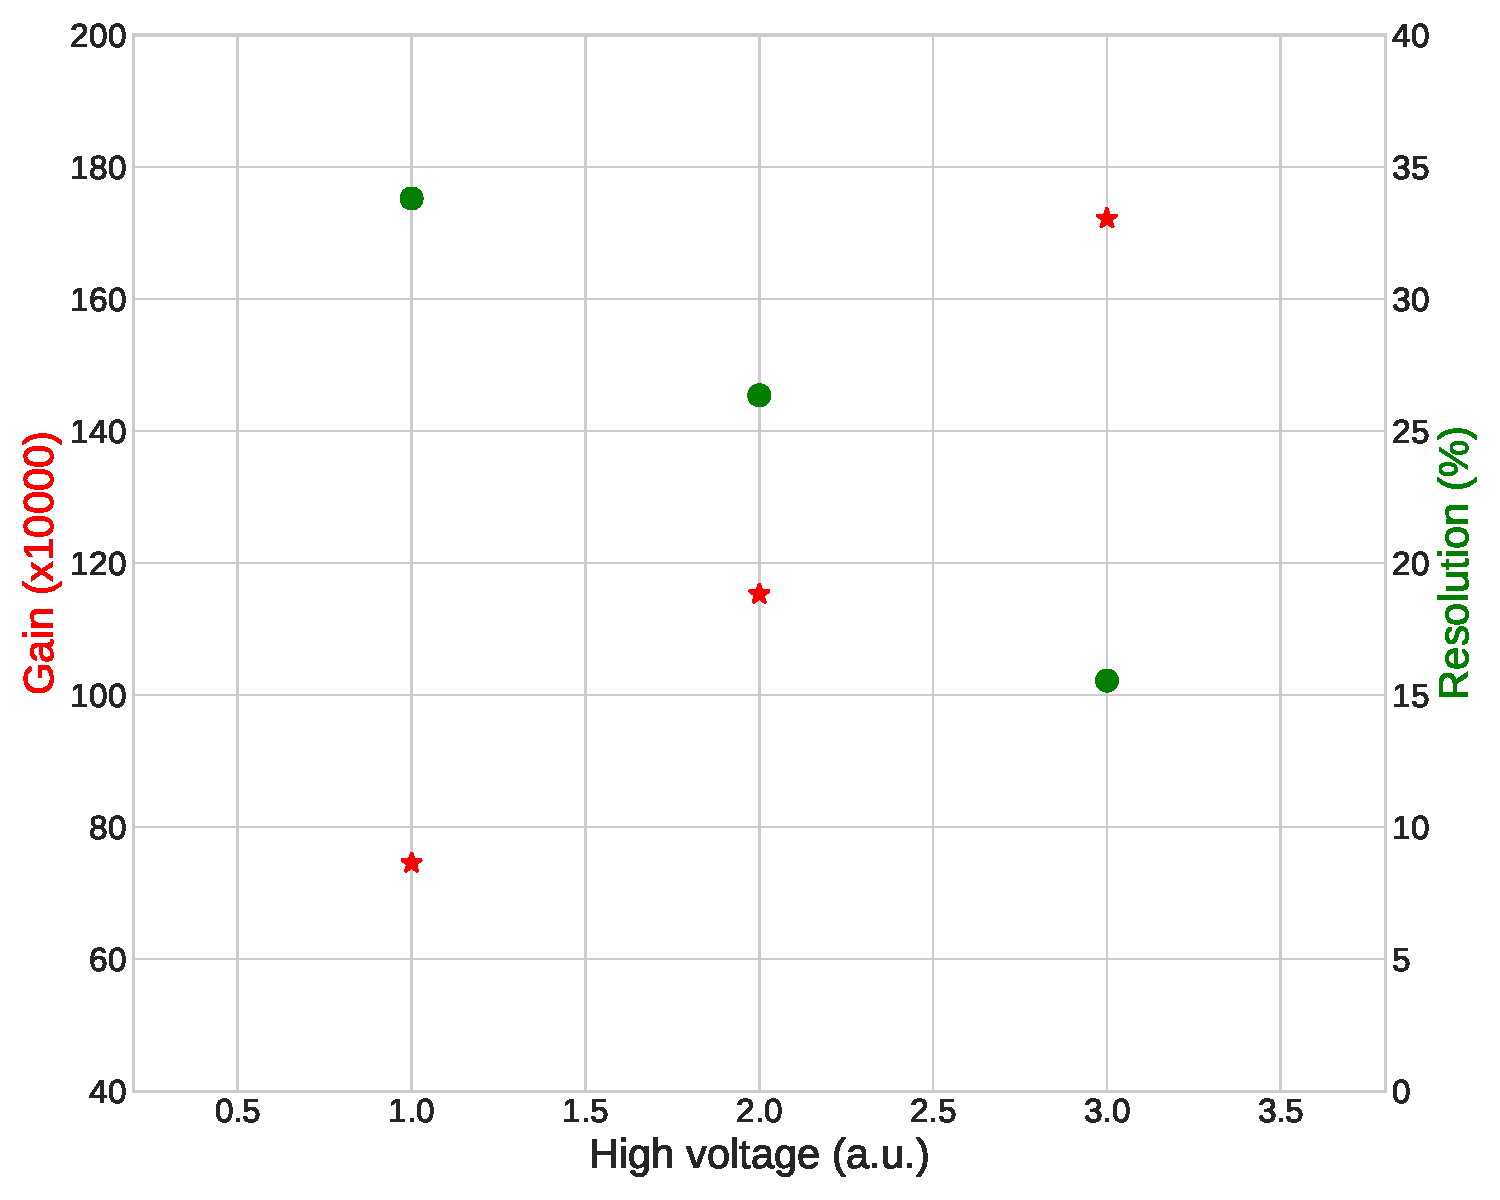
\includegraphics[width=0.7\textwidth]{exampleAnalysis/plots/Electron_Gain_Resolution_HV_VME.pdf}\\}
\end{additional}
}

\pagebreak
